\chapter{Simulation}\label{ch:Simulation}

Simulation was extensively used throughout this thesis due to the complex nature of the systems involved. 

Both hardware, and software simulation was used to understand the performance of the receiver. Hardware simulation involves the C firmware being run on the \ac{NAMURU} processor, while a Spirent GNSS simulator is used to generate a RF signal. Software simulation involves a Python model of the tracking loops being tested using synthetic data generated in software. Both forms of simulation are complementary. Hardware simulations being the most representative of the true performance of the receiver, however they run in real time, require a \$250,000 GNSS simulator and it can be difficult to observe the state of the tracking loops without disturbing them. Conversely, software simulations are significantly cheaper, as they run entirely on a computer. Additionally, the simulation can run as fast as the computational hardware will allow, typically 100 faster $\times$ faster. Finally, the state of the receiver can be measured without affecting the performance of the receiver.

\subsection{Hardware simulation}
The state of the receiver can be determined, both on a gross basis via NMEA output from the receiver, or on a finer basis by using the KeaDebug feature. KeaDebug collects information about the internal state of the receiver, including the doppler frequency, phase angle, tracking mode and I and Q values. These values are then transmitted to a tethered laptop, where they can be stored for further analysis. One of the downsides of using the KeaDebug feature, is the potential to increase the computational load faced by the receiver. This in turn can lead to an increase in the timing jitter for collecting samples and updating the loops, which in turn increases the phase jitter. 

In particular, collecting I\&Q samples increases the computational load by 47\%, leading to the perverse phenomenon that attempting to collect more information regarding regarding the receivers performance, leads to a degrade in performance.

\begin{table}[!htb]
\centering
\begin{tabular}{|l|l|}
\hline
\rowcolor[HTML]{C0C0C0} 
Address & Variable                                                             \\ \hline
100     & VE, E, P and L amplitudes                                            \\ \hline
\rowcolor[HTML]{EFEFEF} 
110     & Doppler frequency (units of Hz)                                      \\ \hline
120     & Delay error (Chips x 1000 )                                          \\ \hline
\rowcolor[HTML]{EFEFEF} 
130     & Channel status (1 = searching, 2 = capturing, 3 = tracking)          \\ \hline
140     & Carrier tracking mode (1 = code lock, 2 = freq lock, 3 = phase lock) \\ \hline
\rowcolor[HTML]{EFEFEF} 
150     & Satellite number                                                     \\ \hline
190     & Detected flag (1=detected, 0=not detected                            \\ \hline
\rowcolor[HTML]{EFEFEF} 
230     & Phase angle (cycles x 1024)                                          \\ \hline
240     & Differential phase angle (cycles x 1024)                             \\ \hline
\rowcolor[HTML]{EFEFEF} 
260     & Detection threshold                                                  \\ \hline
270     & False frequency metric                                               \\ \hline
\rowcolor[HTML]{EFEFEF} 
280     & Coherent integration period (4 ms when tracking)                     \\ \hline
290     & Number of non-coherent rounds (8 when tracking)                      \\ \hline
\rowcolor[HTML]{EFEFEF} 
340     & Prompt in-phase sample (I)                                           \\ \hline
350     & Prompt quadrature phase sample (Q)                                   \\ \hline
\end{tabular}
\caption{KeaDebug variables avalible for dumping to a host computer.}
\label{tab:KeaDebugKey}
\end{table}

\begin{figure}[!htb] 
    \centering
    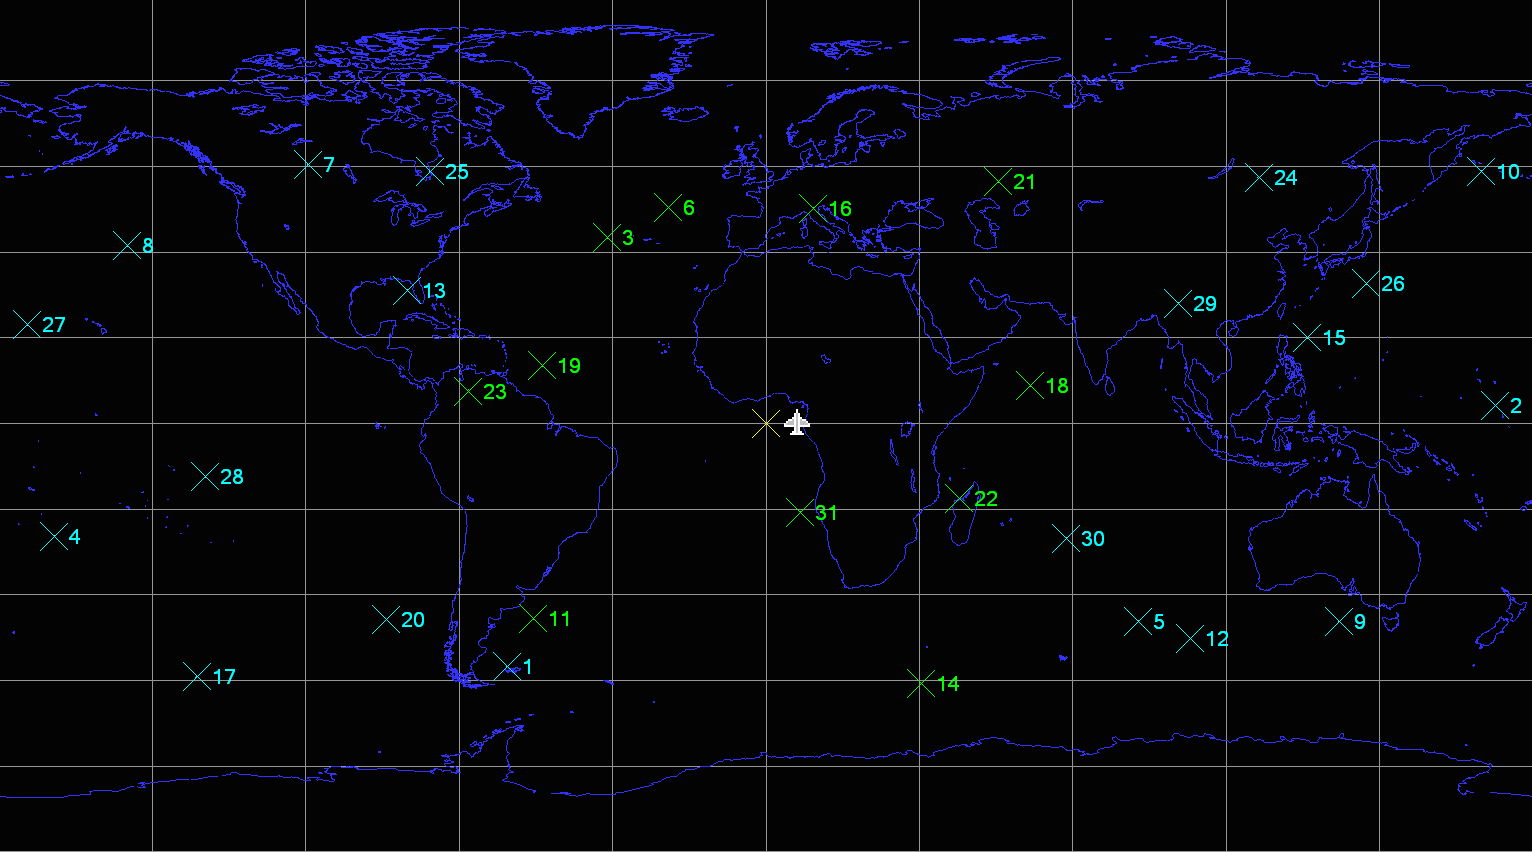
\includegraphics[width=1\textwidth]{Simulation/SpirentSatelliteMap.png} 
    \caption{A map of the receiver's simulated location and positions of the satellites in the GPS constellation. Satellites that are currently in view of the receiver are displayed in green, with satellites below the horizon in cyan.}
    \label{fig:SpirentSatelliteMap}
\end{figure}



\begin{figure}[!htb] 
    \centering
    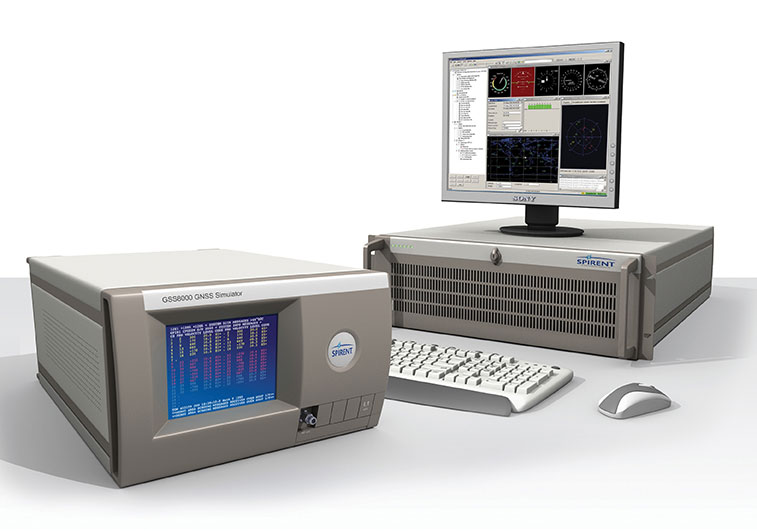
\includegraphics[width=1\textwidth]{mywork/Spirent-GSS8000.jpg} 
    \caption{An example of a Spirent \ac{GPS} simulator. The actual model used for this research differs from the one pictured. The simulator is controlled by a tethered computer, which runs the \emph{SimGen} software, pictured in figure \ref{:HighGScreenshot}.}
    \label{fig:Spirent}
\end{figure}

\begin{figure}[!htb] 
    \centering
    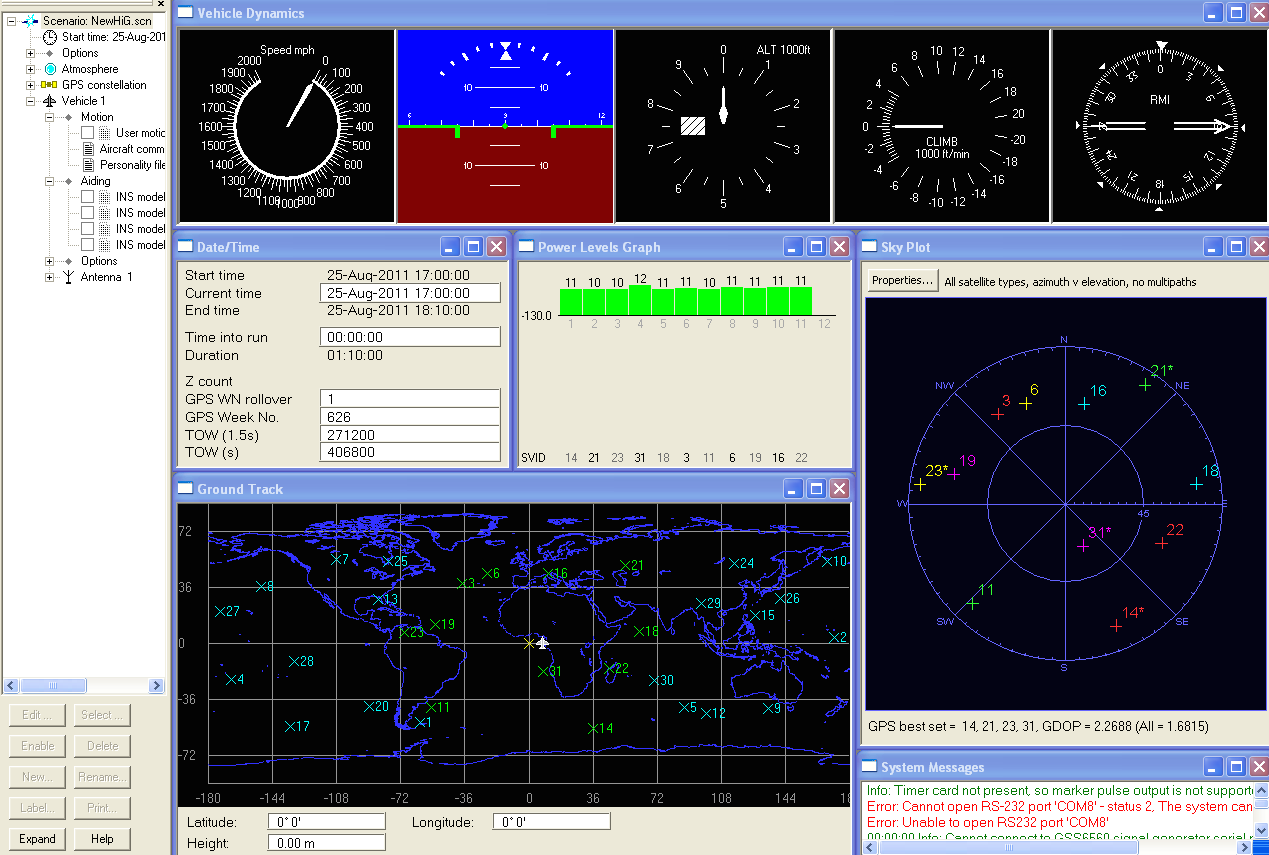
\includegraphics[width=1\textwidth]{mywork/HighGScreenshot.png} 
    \caption{The SimGen software, used to define scenarios and control the \ac{GNSS} simulator.}
    \label{:HighGScreenshot}
\end{figure}


The correct performance of a \ac{PLL} can be determined in a number of ways. The receiver internally uses a lock detection algorithm to decided which state it is currently in, and which set of tracking loops should be used. The current state is can be determined by examining the output from the KeaDebug. Another method that was employed to verify the correct operation of the software receiver is to observe the raw I \& Q values. In the case that the receiver is truly in phase lock with the incoming signal, the binary bit-stream transmitted by the satellite can be observed in the prompt I values. In figure \ref{fig:DigitalData} the decoded message can be clearly seen, indicating that the receiver is maintaining phase lock with the signal. 

\begin{figure}[!htb] 
    \centering
    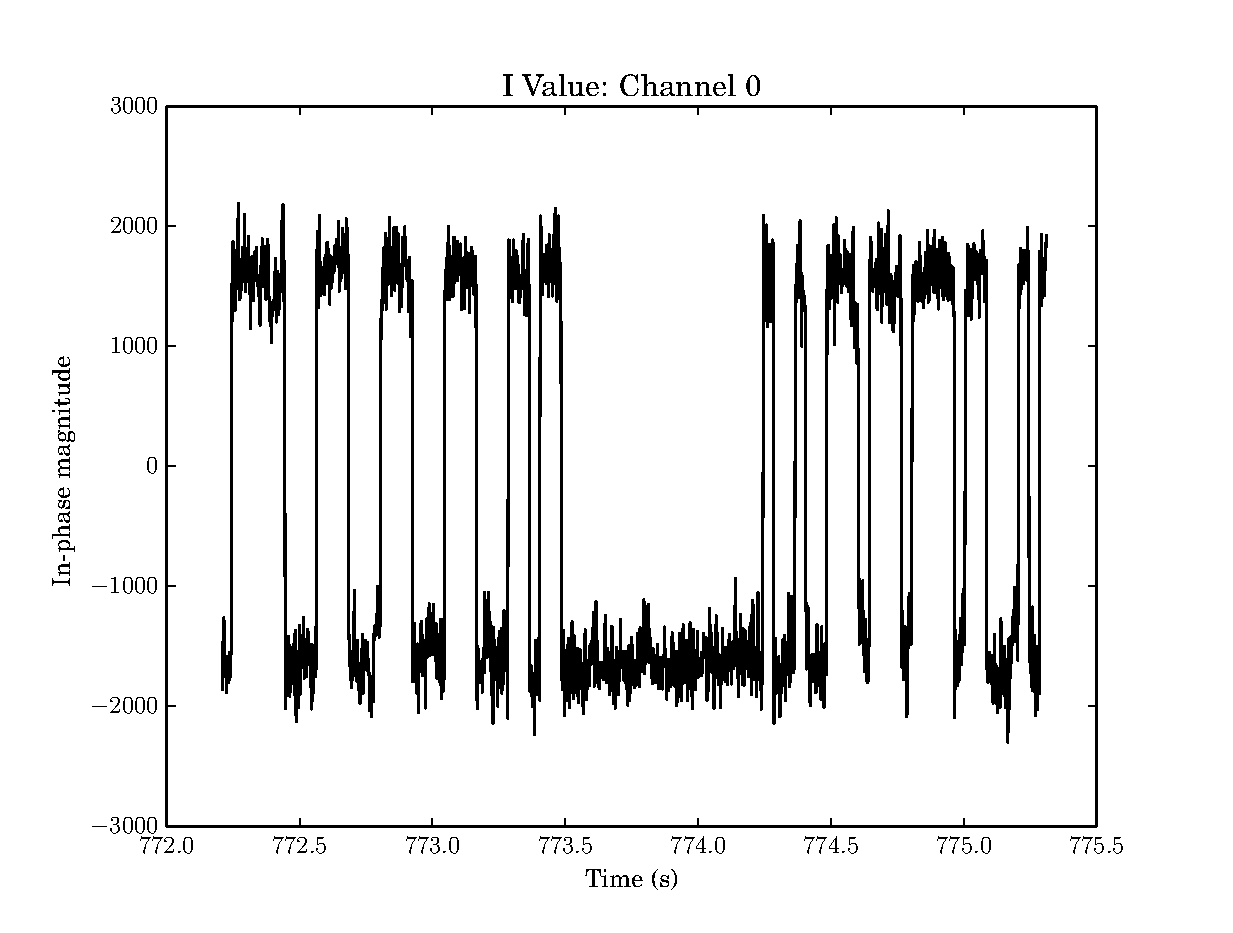
\includegraphics[width=1\textwidth]{Simulation/DigitalData.eps} 
    \caption{The 50 bps digital signal decoded from the phase modulated signal from the satellite.}
    \label{fig:DigitalData}
\end{figure}



\subsection{HighG3}
The scenario \emph{HighG3} is designed to expose the receiver to dynamics that are far in excess of what will ever be experienced during launch. The peak dynamics experienced are summarised in table \ref{tab:HighG3PeakDynamics}, with the exact sequence of steps in table \ref{tab:HighG3Steps}. The long periods of acceleration are designed to ensure that any errors that cause failure by accumulation over time become apparent. 


\begin{table}[]
\centering
\begin{tabular}{|l|l|l|}
\hline
\rowcolor[HTML]{C0C0C0} 
Derivative   & Value    & Time  \\ \hline
Velocity     & 9,000m/s & n/a   \\ \hline
\rowcolor[HTML]{EFEFEF} 
Acceleration & 150m/s   & 120s  \\ \hline
Jerk         & 500m/s   & 300ms \\ \hline
\end{tabular}
\caption{The peak dynamics experienced during the HighG3 scenario.}
\label{tab:HighG3PeakDynamics}
\end{table}

\begin{table}[]
\centering
\begin{tabular}{|l|l|}
\hline
\rowcolor[HTML]{C0C0C0} 
Time (s) & Action               \\ \hline
0        & Stationary           \\ \hline
\rowcolor[HTML]{EFEFEF} 
900      & 40m/s acceleration east   \\ \hline
960      & Hold 2,400m/s        \\ \hline
\rowcolor[HTML]{EFEFEF} 
970      & -40m/s acceleration east \\ \hline
1030     & Hold 0 m/s           \\ \hline
\rowcolor[HTML]{EFEFEF} 
1050     & 45m/s acceleration  west \\ \hline
\ldots   & \ldots               \\ \hline
\rowcolor[HTML]{EFEFEF} 
4050     & 150m/s acceleration west \\ \hline
4110     & Hold 9,000m/s        \\ \hline
\rowcolor[HTML]{EFEFEF} 
4120     & -150m/s acceleration east\\ \hline
4180     & Hold 0 m/s           \\ \hline
\end{tabular}
\caption{The sequence of dynamics experienced by the receiver. The total run-time of the simulation is approximately 75m including setup time, consisting of 22 separate rounds of acceleration in 5$m/s^2$ intervals.}
\label{tab:HighG3Steps}
\end{table}

It is important to note that these are the accelerations applied to the receiver, as opposed to the \ac{LOS} dynamics experienced, which are significantly less. By observing figure \ref{fig:SpirentSatelliteMap} it is possible to identify that satellites 


\subsection{Software simulation}

A software based receiver has been developed as part of the thesis, in order to gain a greater understanding of the performance of tracking loops on real world data. A significant proportion of the code can be found in appendix \ref{ch:Code}.

The software receiver was developed in Python, based on the authors previous experience with the language, as well the need to interface with domain specific libraries.  The approach of using an \ac{GNSS}, and testing in software was effectively used by Kazemi \cite{KazemiPHD} in order to critically evaluate the performance of the new tracking loops developed as part of his PHD. Ward also used Monte Carlo simulations in order to ascertain the performance limits of his FLL/PLL combined tracking loop.

A signal was generated by a Spirent \ac{GPS} simulator, which can be seen in figure \ref{fig:Spirent}. This signal was then digitised using a NordNav \ac{SDR}, with a sampling rate of $16.3676 \times 10^6$ samples per second. 

A range of simulations were created in order to better understand the performance of the software receiver. In particular, scenarios for 0g, 1g, 2g, 5g, 7.5g and 10g were created. In figure \ref{fig:Doppler}, the output from the \ac{NCO} of the software receiver can be seen. In the simulation, the receiver remains stationary until 8s, at which point it starts accelerating directly upwards at 10g, creating a ramp in the \ac{NCO} frequency. It is important to note that while the receiver is accelerating at 10g, the \ac{LOS} dynamics may only be 5g. 


\section{Airborne experiment}

\begin{figure}[!htb] 
    \centering
    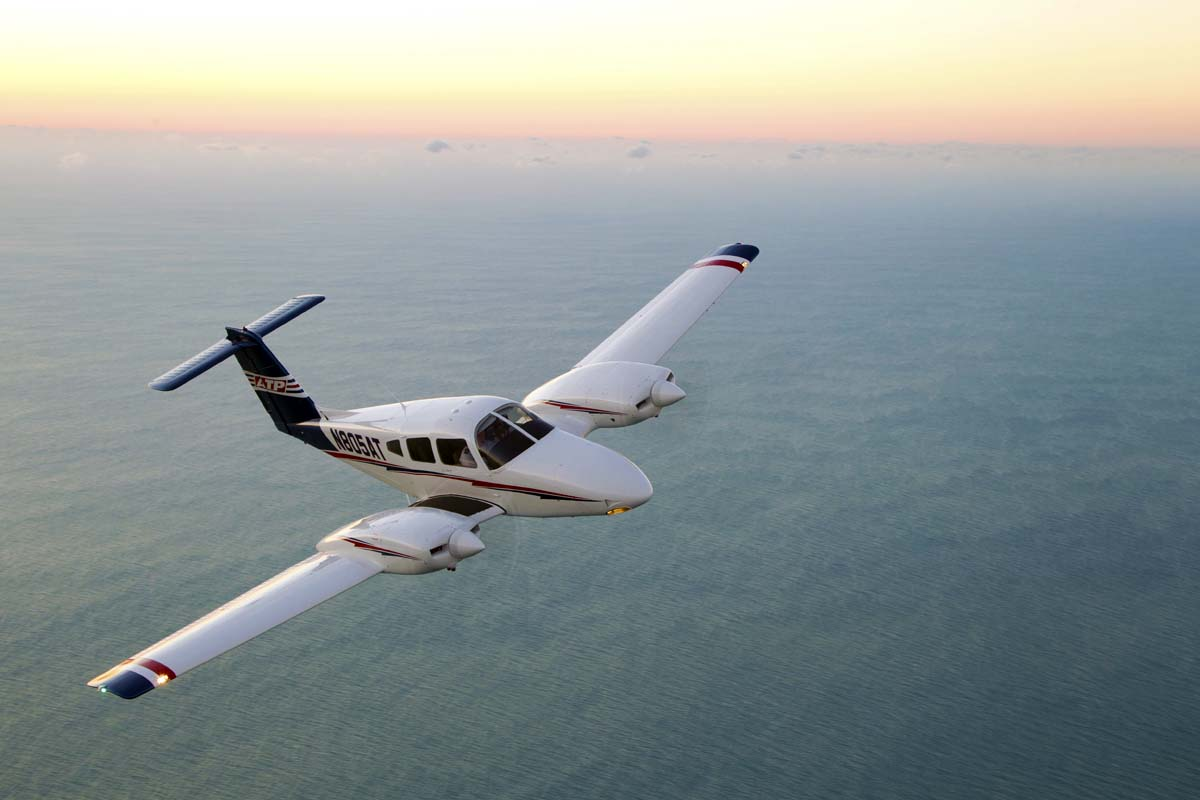
\includegraphics[width=1\textwidth]{mywork/SeminoleBankingPRjpg.jpg} 
    \caption{A Piper PA-44 Seminole.}
    \label{fig:PiperSeminole}
\end{figure}

A real-world data-set was processed, consisting of data taken captured a flight aboard a UNSW Aviation Piper PA-44 Seminole VH-FRI. Data from the flight was captured by a NordNav IF Recorder, and processed using the the software receiver. 

The actual carrier doppler shift, as measured by taking the finite difference of the satellite pseudoranges, and converted to Hz, was compared against the measured Doppler shift in the software receiver. There is a small offset because of drift in the receiver crystal. The results of this experiment can be see in figure \ref{fig:SimulatedDynamics}. While the dynamics experienced by the receiver were on the order of $\pm 5m/s^2$, somewhat less than the dynamics that are experienced by a \ac{LV}, This experiment is important, as it verifies the real world performance of the soft receiver. 


